\documentclass[12pt,a4paper]{article}

% ── Packages ──────────────────────────────────────────────────
\usepackage[utf8]{inputenc}
\usepackage[T1]{fontenc}
\usepackage{geometry}
\geometry{margin=2.5cm}
\usepackage{graphicx}
\usepackage{booktabs}
\usepackage{longtable}
\usepackage{listings}
\usepackage{xcolor}
\usepackage{hyperref}
\usepackage{tikz}
\usetikzlibrary{positioning}
\usepackage{fancyhdr}
\usepackage{titlesec}
\usepackage{enumitem}
\usepackage{caption}
\usepackage{float}

% ── Colors ────────────────────────────────────────────────────
\definecolor{codegreen}{rgb}{0.25,0.49,0.37}
\definecolor{codegray}{rgb}{0.5,0.5,0.5}
\definecolor{codepurple}{rgb}{0.58,0,0.82}
\definecolor{backcolour}{rgb}{0.95,0.95,0.96}
\definecolor{embbgreen}{HTML}{73BF69}
\definecolor{urllcyellow}{HTML}{F2CC0C}
\definecolor{mmtcorange}{HTML}{FF9830}
\definecolor{darkblue}{HTML}{1a237e}

% ── Code listing style ────────────────────────────────────────
\lstdefinestyle{terminal}{
    backgroundcolor=\color{backcolour},
    commentstyle=\color{codegreen},
    keywordstyle=\color{codepurple},
    numberstyle=\tiny\color{codegray},
    stringstyle=\color{codegreen},
    basicstyle=\ttfamily\footnotesize,
    breakatwhitespace=false,
    breaklines=true,
    captionpos=b,
    keepspaces=true,
    showspaces=false,
    showstringspaces=false,
    showtabs=false,
    tabsize=2,
    frame=single,
    rulecolor=\color{codegray},
    xleftmargin=1em,
    framexleftmargin=0.5em,
}

\lstdefinestyle{yaml}{
    backgroundcolor=\color{backcolour},
    basicstyle=\ttfamily\footnotesize,
    breaklines=true,
    frame=single,
    rulecolor=\color{codegray},
    xleftmargin=1em,
    framexleftmargin=0.5em,
    keywordstyle=\color{darkblue},
    stringstyle=\color{codegreen},
    commentstyle=\color{codegray},
}

\lstset{style=terminal}

% ── Header/Footer ─────────────────────────────────────────────
\pagestyle{fancy}
\fancyhf{}
\fancyhead[L]{\footnotesize Two-VM UPF Kubernetes Deployment}
\fancyhead[R]{\footnotesize \today}
\fancyfoot[C]{\thepage}
\renewcommand{\headrulewidth}{0.4pt}

% ── Title formatting ──────────────────────────────────────────
\titleformat{\section}{\Large\bfseries\color{darkblue}}{\thesection}{1em}{}
\titleformat{\subsection}{\large\bfseries\color{darkblue!80}}{\thesubsection}{1em}{}
\titleformat{\subsubsection}{\normalsize\bfseries\color{darkblue!60}}{\thesubsubsection}{1em}{}

\hypersetup{
    colorlinks=true,
    linkcolor=darkblue,
    urlcolor=darkblue!70,
    citecolor=darkblue,
}

% ══════════════════════════════════════════════════════════════
\begin{document}

% ── Title Page ────────────────────────────────────────────────
\begin{titlepage}
\centering
\vspace*{3cm}

{\Huge\bfseries\color{darkblue} Two-VM UPF Kubernetes\\[0.3em] Deployment Report}

\vspace{1.5cm}

{\Large Cloud-Native 5G Network Slicing with\\Prometheus \& Grafana Monitoring}

\vspace{2cm}

\begin{tabular}{ll}
\toprule
\textbf{Parameter} & \textbf{Value} \\
\midrule
VM1 (Control Plane) & 192.168.49.143 \\
VM2 (Data Plane — Kubernetes) & 192.168.49.171 \\
VM3 (RAN — gNB + UEs) & 192.168.49.139 \\
Date & \today \\
\bottomrule
\end{tabular}

\vspace{3cm}

{\large 5G Core: Open5GS \quad|\quad RAN: UERANSIM \quad|\quad Orchestration: Kubernetes (Minikube)}

\vfill
\end{titlepage}

% ── Table of Contents ─────────────────────────────────────────
\tableofcontents
\newpage

% ══════════════════════════════════════════════════════════════
\section{Architecture Overview}
% ══════════════════════════════════════════════════════════════

The deployment follows a \textbf{two-VM architecture} separating the 5G control plane from the data plane:

\begin{itemize}[leftmargin=2em]
    \item \textbf{VM1 (192.168.49.143)} — Control Plane: AMF, NRF, SMF (×3), UDM, UDR, PCF, AUSF, BSF, MongoDB
    \item \textbf{VM2 (192.168.49.171)} — Data Plane: UPF pods (×3) running in Kubernetes, Prometheus, Grafana
    \item \textbf{VM3 (192.168.49.139)} — RAN: UERANSIM gNB + 3 UE simulators
\end{itemize}

\begin{figure}[H]
\centering
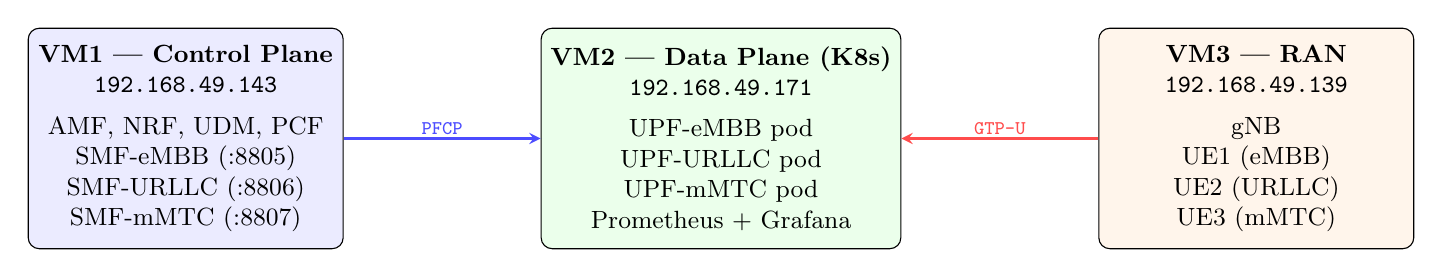
\begin{tikzpicture}[
    node distance=1.5cm,
    box/.style={draw, rounded corners, minimum width=4cm, minimum height=2.8cm, align=center, font=\small},
    arrow/.style={->, >=stealth, thick},
    label/.style={font=\scriptsize\ttfamily, fill=white, inner sep=1pt},
]
    % VM1
    \node[box, fill=blue!8] (vm1) {
        \textbf{VM1 — Control Plane}\\
        \texttt{192.168.49.143}\\[4pt]
        AMF, NRF, UDM, PCF\\
        SMF-eMBB (:8805)\\
        SMF-URLLC (:8806)\\
        SMF-mMTC (:8807)
    };
    % VM2
    \node[box, fill=green!8, right=2.5cm of vm1] (vm2) {
        \textbf{VM2 — Data Plane (K8s)}\\
        \texttt{192.168.49.171}\\[4pt]
        UPF-eMBB pod\\
        UPF-URLLC pod\\
        UPF-mMTC pod\\
        Prometheus + Grafana
    };
    % VM3
    \node[box, fill=orange!8, right=2.5cm of vm2] (vm3) {
        \textbf{VM3 — RAN}\\
        \texttt{192.168.49.139}\\[4pt]
        gNB\\
        UE1 (eMBB)\\
        UE2 (URLLC)\\
        UE3 (mMTC)
    };
    % Arrows
    \draw[arrow, blue!70] (vm1) -- node[label, above] {PFCP} (vm2);
    \draw[arrow, red!70] (vm3) -- node[label, above] {GTP-U} (vm2);
\end{tikzpicture}
\caption{Two-VM UPF Kubernetes Architecture}
\end{figure}

\subsection{Network Slice Mapping}

\begin{table}[H]
\centering
\begin{tabular}{lcccccc}
\toprule
\textbf{Slice} & \textbf{Namespace} & \textbf{PFCP Port} & \textbf{GTP-U IP} & \textbf{Subnet} & \textbf{DNN} & \textbf{Shaping} \\
\midrule
\textcolor{embbgreen}{\textbf{eMBB}} & \texttt{embb} & 8805 & 192.168.49.171 & 10.45.0.0/24 & internet & 100 Mbit \\
\textcolor{urllcyellow}{\textbf{URLLC}} & \texttt{urllc} & 8806 & 192.168.49.172 & 10.46.0.0/24 & urllc & 50 Mbit + 1ms \\
\textcolor{mmtcorange}{\textbf{mMTC}} & \texttt{mmtc} & 8807 & 192.168.49.173 & 10.47.0.0/24 & iot & 1 Mbit \\
\bottomrule
\end{tabular}
\caption{Per-Slice Network Configuration}
\end{table}


% ══════════════════════════════════════════════════════════════
\section{File Inventory}
% ══════════════════════════════════════════════════════════════

\begin{lstlisting}[style=terminal, title=Project Structure]
/home/kube/kubernetes/
|-- k8s/
|   |-- Dockerfile                     # UPF container image
|   |-- entrypoint.sh                  # TUN + NAT + tc shaping
|   |-- embb/upf-embb.yaml            # eMBB ConfigMap + Deployment
|   |-- urllc/upf-urllc.yaml          # URLLC ConfigMap + Deployment
|   |-- mmtc/upf-mmtc.yaml            # mMTC ConfigMap + Deployment
|   +-- monitoring/
|       |-- namespace.yaml             # monitoring namespace
|       |-- tun-metrics-exporter.yaml  # Python exporter DaemonSet
|       |-- prometheus.yaml            # Prometheus Deployment
|       +-- grafana.yaml               # Grafana + Dashboard JSON
+-- open5gs/
    |-- smf-embb.yaml                  # SMF configs (VM1)
    |-- smf-urllc.yaml
    +-- smf-mmtc.yaml
\end{lstlisting}


% ══════════════════════════════════════════════════════════════
\section{Step 1 — Fix UPF Pods (CrashLoopBackOff)}
% ══════════════════════════════════════════════════════════════

\subsection{Problem}

All 3 UPF pods were crashing with \texttt{Cannot assign requested address}. The Kubernetes ConfigMaps had \textbf{stale addresses} from a previous deployment on VM1 (loopback addresses and VM1 IPs) that do not exist on VM2.

\begin{table}[H]
\centering
\begin{tabular}{lllll}
\toprule
\textbf{Slice} & \textbf{Stale PFCP} & \textbf{Stale GTP-U} & \textbf{Correct PFCP} & \textbf{Correct GTP-U} \\
\midrule
eMBB  & \texttt{127.0.0.7:8805} & \texttt{192.168.49.143:2152} & \texttt{192.168.49.171:8805} & \texttt{192.168.49.171:2152} \\
URLLC & \texttt{127.0.0.8:8806} & \texttt{192.168.49.144:2152} & \texttt{192.168.49.171:8806} & \texttt{192.168.49.172:2152} \\
mMTC  & \texttt{127.0.0.9:8807} & \texttt{192.168.49.146:2152} & \texttt{192.168.49.171:8807} & \texttt{192.168.49.173:2152} \\
\bottomrule
\end{tabular}
\caption{Stale vs.\ Correct UPF Addresses}
\end{table}

\subsection{Error Logs (Before Fix)}

\begin{lstlisting}[style=terminal]
[pfcp] INFO: pfcp_server() [127.0.0.7]:8805
[sock] ERROR: socket bind(2) [192.168.49.143]:2152 failed
       (99:Cannot assign requested address)
[app] FATAL: Open5GS initialization failed. Aborted
\end{lstlisting}

\subsection{Fix — Re-apply Manifests and Restart Pods}

\begin{lstlisting}[style=terminal]
# Re-apply to update ConfigMaps with correct addresses
kubectl apply -f /home/kube/kubernetes/k8s/embb/upf-embb.yaml
kubectl apply -f /home/kube/kubernetes/k8s/urllc/upf-urllc.yaml
kubectl apply -f /home/kube/kubernetes/k8s/mmtc/upf-mmtc.yaml

# Restart pods to pick up new ConfigMap values
kubectl rollout restart deployment/upf-embb  -n embb
kubectl rollout restart deployment/upf-urllc -n urllc
kubectl rollout restart deployment/upf-mmtc  -n mmtc
\end{lstlisting}

\subsection{Result — All Pods Running}

\begin{lstlisting}[style=terminal]
NAMESPACE   NAME                         READY   STATUS    AGE
embb        upf-embb-68d8c9bc9-l2745    1/1     Running   24s
urllc       upf-urllc-7fbf49c66c-xw5fs  1/1     Running   24s
mmtc        upf-mmtc-84f689d5f5-ln9r7   1/1     Running   24s
\end{lstlisting}

\subsection{Verified PFCP Associations}

After restart, all 3 UPFs established PFCP associations with their corresponding SMFs on VM1:

\begin{lstlisting}[style=terminal]
eMBB:  pfcp_server() [192.168.49.171]:8805
       gtp_server()  [192.168.49.171]:2152
       PFCP associated [192.168.49.143]:8805

URLLC: pfcp_server() [192.168.49.171]:8806
       gtp_server()  [192.168.49.172]:2152
       PFCP associated [192.168.49.143]:8806

mMTC:  pfcp_server() [192.168.49.171]:8807
       gtp_server()  [192.168.49.173]:2152
       PFCP associated [192.168.49.143]:8807
\end{lstlisting}


% ══════════════════════════════════════════════════════════════
\section{Step 2 — Fix iptables FORWARD Chain}
% ══════════════════════════════════════════════════════════════

\subsection{Problem}

End-to-end \texttt{ping} from VM3 (UE) to the internet failed. Docker's default iptables FORWARD chain had \texttt{policy DROP}, blocking traffic from UPF TUN interfaces (\texttt{ogstun-*}) to the external interface (\texttt{ens33}).

\begin{lstlisting}[style=terminal]
Chain FORWARD (policy DROP)
  ... DOCKER-USER, DOCKER-FORWARD, KUBE-* ...
  # No rules for ogstun-* traffic -> DROPPED
\end{lstlisting}

\subsection{Fix — Add FORWARD Rules}

\begin{lstlisting}[style=terminal]
# Allow outbound: ogstun-* -> ens33
sudo iptables -I FORWARD 1 -i ogstun-embb  -o ens33 -j ACCEPT
sudo iptables -I FORWARD 1 -i ogstun-urllc -o ens33 -j ACCEPT
sudo iptables -I FORWARD 1 -i ogstun-mmtc  -o ens33 -j ACCEPT

# Allow return traffic: ens33 -> ogstun-*
sudo iptables -I FORWARD 1 -i ens33 -o ogstun-embb  \
    -m state --state RELATED,ESTABLISHED -j ACCEPT
sudo iptables -I FORWARD 1 -i ens33 -o ogstun-urllc \
    -m state --state RELATED,ESTABLISHED -j ACCEPT
sudo iptables -I FORWARD 1 -i ens33 -o ogstun-mmtc  \
    -m state --state RELATED,ESTABLISHED -j ACCEPT
\end{lstlisting}

\textbf{Note:} These rules are \emph{not persistent} across reboots. For persistence, add them to \texttt{entrypoint.sh} or a systemd unit.


% ══════════════════════════════════════════════════════════════
\section{Step 3 — End-to-End Verification}
% ══════════════════════════════════════════════════════════════

\subsection{Traffic Tests (from VM1)}

Three tests were conducted, one per slice, from the VM hosting the UE simulators:

\begin{lstlisting}[style=terminal]
# eMBB - YouTube/web traffic (high bandwidth)
curl --interface uesimtun0 https://www.youtube.com

# URLLC - Low-latency small packets
ping -I uesimtun1 -s 64 -i 0.01 8.8.8.8

# mMTC - IoT sensor simulation
curl --interface uesimtun2 -X POST https://httpbin.org/post \
    -d '{"sensor":"temp","value":22.5}'
\end{lstlisting}

All three tests completed successfully.

\subsection{Traffic Counters on VM2}

\begin{table}[H]
\centering
\begin{tabular}{lrrrrc}
\toprule
\textbf{Interface} & \textbf{RX bytes} & \textbf{RX pkts} & \textbf{TX bytes} & \textbf{TX pkts} & \textbf{Errors} \\
\midrule
\texttt{ogstun-embb}  & 23,589  & 534   & 754,989 & 674   & 0 \\
\texttt{ogstun-urllc} & 172,412 & 1,877 & 194,012 & 1,997 & 0 \\
\texttt{ogstun-mmtc}  & 4,766   & 50    & 35,007  & 171   & 0 \\
\bottomrule
\end{tabular}
\caption{TUN Interface Counters After Traffic Tests}
\end{table}

\subsection{Secondary IPs on VM2}

URLLC and mMTC UPFs use dedicated secondary IPs for GTP-U to enable per-slice traffic separation:

\begin{lstlisting}[style=terminal]
sudo ip addr add 192.168.49.172/24 dev ens33   # URLLC GTP-U
sudo ip addr add 192.168.49.173/24 dev ens33   # mMTC GTP-U
\end{lstlisting}

Verification:
\begin{lstlisting}[style=terminal]
inet 192.168.49.171/24  scope global dynamic ens33      # eMBB
inet 192.168.49.172/24  scope global secondary ens33     # URLLC
inet 192.168.49.173/24  scope global secondary ens33     # mMTC
\end{lstlisting}


% ══════════════════════════════════════════════════════════════
\section{Step 4 — Monitoring Stack Deployment}
% ══════════════════════════════════════════════════════════════

\subsection{Overview}

Since Open5GS UPF does not expose native Prometheus metrics, a custom \textbf{TUN Metrics Exporter} was built to read kernel-level interface statistics and expose them in Prometheus format.

\begin{figure}[H]
\centering
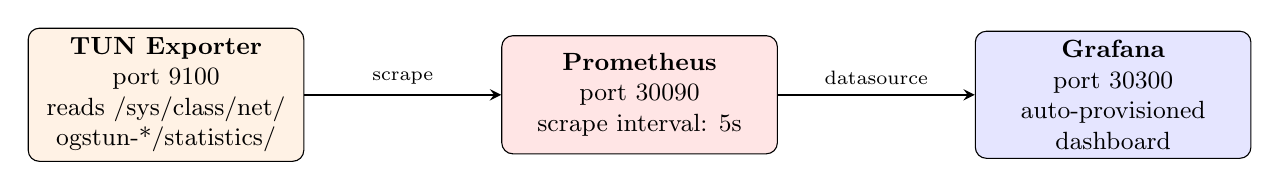
\begin{tikzpicture}[
    node distance=2cm,
    box/.style={draw, rounded corners, minimum width=3.5cm, minimum height=1.5cm, align=center, font=\small},
    arrow/.style={->, >=stealth, thick},
]
    \node[box, fill=orange!10] (exporter) {\textbf{TUN Exporter}\\port 9100\\reads /sys/class/net/\\ogstun-*/statistics/};
    \node[box, fill=red!10, right=2.5cm of exporter] (prom) {\textbf{Prometheus}\\port 30090\\scrape interval: 5s};
    \node[box, fill=blue!10, right=2.5cm of prom] (grafana) {\textbf{Grafana}\\port 30300\\auto-provisioned\\dashboard};

    \draw[arrow] (exporter) -- node[above, font=\scriptsize] {scrape} (prom);
    \draw[arrow] (prom) -- node[above, font=\scriptsize] {datasource} (grafana);
\end{tikzpicture}
\caption{Monitoring Pipeline}
\end{figure}

\subsection{TUN Metrics Exporter}

A Python script deployed as a Kubernetes \texttt{DaemonSet} that reads TUN interface statistics from \texttt{/sys/class/net/ogstun-*/statistics/} and serves Prometheus-format metrics on port 9100.

\begin{table}[H]
\centering
\begin{tabular}{lll}
\toprule
\textbf{Metric} & \textbf{Labels} & \textbf{Description} \\
\midrule
\texttt{tun\_rx\_bytes}   & interface, slice & Bytes received on TUN \\
\texttt{tun\_tx\_bytes}   & interface, slice & Bytes transmitted on TUN \\
\texttt{tun\_rx\_packets} & interface, slice & Packets received \\
\texttt{tun\_tx\_packets} & interface, slice & Packets transmitted \\
\texttt{tun\_rx\_errors}  & interface, slice & Receive errors \\
\texttt{tun\_tx\_errors}  & interface, slice & Transmit errors \\
\texttt{tun\_rx\_dropped} & interface, slice & Receive drops \\
\texttt{tun\_tx\_dropped} & interface, slice & Transmit drops \\
\bottomrule
\end{tabular}
\caption{Prometheus Metrics Exposed by TUN Exporter}
\end{table}

\subsection{Prometheus}

\begin{itemize}
    \item \textbf{Image:} \texttt{prom/prometheus:v2.51.0}
    \item \textbf{Scrape interval:} 5 seconds
    \item \textbf{Target:} \texttt{192.168.49.171:9100} (TUN exporter)
    \item \textbf{Access:} \texttt{http://192.168.49.171:30090}
    \item \textbf{Retention:} 7 days
\end{itemize}

\subsection{Grafana}

\begin{itemize}
    \item \textbf{Image:} \texttt{grafana/grafana:10.4.1}
    \item \textbf{Access:} \texttt{http://192.168.49.171:30300}
    \item \textbf{Credentials:} admin / admin
    \item \textbf{Datasource:} Prometheus (auto-provisioned)
    \item \textbf{Dashboard:} ``5G Network Slice Monitor'' (auto-loaded as home)
\end{itemize}

\subsection{Deployment Commands}

\begin{lstlisting}[style=terminal]
kubectl apply -f k8s/monitoring/namespace.yaml
kubectl apply -f k8s/monitoring/tun-metrics-exporter.yaml
kubectl apply -f k8s/monitoring/prometheus.yaml
kubectl apply -f k8s/monitoring/grafana.yaml
\end{lstlisting}

\subsection{Pod Status}

\begin{lstlisting}[style=terminal]
NAMESPACE    NAME                             READY  STATUS
monitoring   tun-metrics-exporter-lt7pc       1/1    Running
monitoring   prometheus-66585fc459-pxmm8      1/1    Running
monitoring   grafana-959684b64-mlrqd          1/1    Running
\end{lstlisting}


% ══════════════════════════════════════════════════════════════
\section{Step 5 — Grafana Dashboard}
% ══════════════════════════════════════════════════════════════

The dashboard ``\textbf{5G Network Slice Monitor}'' contains 9 panels across 4 rows, with each slice assigned a distinct color:

\begin{table}[H]
\centering
\begin{tabular}{cllll}
\toprule
\textbf{Row} & \textbf{Panel} & \textbf{Type} & \textbf{Description} & \textbf{Color} \\
\midrule
1 & eMBB Throughput  & Time series & TX/RX bytes/sec  & \textcolor{embbgreen}{\textbf{Green}} \\
1 & URLLC Throughput & Time series & TX/RX bytes/sec  & \textcolor{urllcyellow}{\textbf{Yellow}} \\
1 & mMTC Throughput  & Time series & TX/RX bytes/sec  & \textcolor{mmtcorange}{\textbf{Orange}} \\
\midrule
2 & eMBB Packet Rate  & Time series & TX/RX pps  & \textcolor{embbgreen}{\textbf{Green}} \\
2 & URLLC Packet Rate & Time series & TX/RX pps  & \textcolor{urllcyellow}{\textbf{Yellow}} \\
2 & mMTC Packet Rate  & Time series & TX/RX pps  & \textcolor{mmtcorange}{\textbf{Orange}} \\
\midrule
3 & Total Traffic     & Stat  & Cumulative bytes per slice & — \\
3 & Live Bandwidth    & Gauge & Real-time bandwidth        & — \\
\midrule
4 & Errors \& Drops   & Time series & RX/TX errors and drops & — \\
\bottomrule
\end{tabular}
\caption{Grafana Dashboard Panel Layout}
\end{table}

% If you have a screenshot, uncomment and adjust:
% \begin{figure}[H]
% \centering
% \includegraphics[width=\textwidth]{grafana_dashboard.png}
% \caption{5G Network Slice Monitor — Grafana Dashboard}
% \end{figure}


% ══════════════════════════════════════════════════════════════
\section{UPF Configuration Details}
% ══════════════════════════════════════════════════════════════

\subsection{eMBB UPF (\texttt{upf-embb.yaml})}

\begin{lstlisting}[style=yaml]
upf:
  pfcp:
    server:
      - address: 192.168.49.171
        port: 8805
  gtpu:
    server:
      - address: 192.168.49.171
        port: 2152
  session:
    - subnet: 10.45.0.0/24
      gateway: 10.45.0.1
      dev: ogstun-embb
      dnn: internet
# tc shaping: 100mbit
\end{lstlisting}

\subsection{URLLC UPF (\texttt{upf-urllc.yaml})}

\begin{lstlisting}[style=yaml]
upf:
  pfcp:
    server:
      - address: 192.168.49.171
        port: 8806
  gtpu:
    server:
      - address: 192.168.49.172    # secondary IP
        port: 2152
  session:
    - subnet: 10.46.0.0/24
      gateway: 10.46.0.1
      dev: ogstun-urllc
      dnn: urllc
# tc shaping: 50mbit + 1ms netem latency
\end{lstlisting}

\subsection{mMTC UPF (\texttt{upf-mmtc.yaml})}

\begin{lstlisting}[style=yaml]
upf:
  pfcp:
    server:
      - address: 192.168.49.171
        port: 8807
  gtpu:
    server:
      - address: 192.168.49.173    # secondary IP
        port: 2152
  session:
    - subnet: 10.47.0.0/24
      gateway: 10.47.0.1
      dev: ogstun-mmtc
      dnn: iot
# tc shaping: 1mbit (ceil 5mbit)
\end{lstlisting}


% ══════════════════════════════════════════════════════════════
\section{SMF Configuration (VM1)}
% ══════════════════════════════════════════════════════════════

All 3 SMFs on VM1 point their PFCP clients to the UPFs on VM2:

\begin{table}[H]
\centering
\begin{tabular}{llll}
\toprule
\textbf{SMF} & \textbf{Config File} & \textbf{PFCP Server (local)} & \textbf{PFCP Client (UPF on VM2)} \\
\midrule
SMF-eMBB  & \texttt{smf-embb.yaml}  & \texttt{192.168.49.143:8805} & \texttt{192.168.49.171:8805} \\
SMF-URLLC & \texttt{smf-urllc.yaml} & \texttt{192.168.49.143:8806} & \texttt{192.168.49.171:8806} \\
SMF-mMTC  & \texttt{smf-mmtc.yaml}  & \texttt{192.168.49.143:8807} & \texttt{192.168.49.171:8807} \\
\bottomrule
\end{tabular}
\caption{SMF $\leftrightarrow$ UPF PFCP Mapping}
\end{table}


% ══════════════════════════════════════════════════════════════
\section{Complete Kubernetes Resource Summary}
% ══════════════════════════════════════════════════════════════

\begin{lstlisting}[style=terminal]
$ kubectl get all -A --selector=slice
NAMESPACE   NAME                         READY  STATUS   RESTARTS
embb        pod/upf-embb-68d8c9bc9-...  1/1    Running  0
urllc       pod/upf-urllc-7fbf49c66c-.. 1/1    Running  0
mmtc        pod/upf-mmtc-84f689d5f5-... 1/1    Running  0

$ kubectl get all -n monitoring
NAME                             READY  STATUS
tun-metrics-exporter-lt7pc       1/1    Running
prometheus-66585fc459-pxmm8      1/1    Running
grafana-959684b64-mlrqd          1/1    Running

SERVICE                    TYPE       PORT(S)
tun-metrics-exporter       ClusterIP  9100/TCP
prometheus                 NodePort   9090:30090/TCP
grafana                    NodePort   3000:30300/TCP
\end{lstlisting}


% ══════════════════════════════════════════════════════════════
\section{Access Points}
% ══════════════════════════════════════════════════════════════

\begin{table}[H]
\centering
\begin{tabular}{ll}
\toprule
\textbf{Service} & \textbf{URL} \\
\midrule
Grafana Dashboard  & \url{http://192.168.49.171:30300} \\
Prometheus UI      & \url{http://192.168.49.171:30090} \\
TUN Metrics (raw)  & \url{http://192.168.49.171:9100/metrics} \\
\bottomrule
\end{tabular}
\caption{Service Access Points}
\end{table}


% ══════════════════════════════════════════════════════════════
\section{Conclusion}
% ══════════════════════════════════════════════════════════════

The two-VM UPF Kubernetes deployment was successfully completed with the following achievements:

\begin{enumerate}
    \item \textbf{Control/Data Plane Separation} — SMFs run on VM1 while UPFs run as Kubernetes pods on VM2, connected via PFCP over the 192.168.49.0/24 network.
    \item \textbf{Three Network Slices} — eMBB (high bandwidth), URLLC (low latency), and mMTC (IoT) slices are fully operational with namespace-level isolation and per-slice traffic shaping.
    \item \textbf{End-to-End Connectivity} — UE traffic from VM3 traverses the gNB (GTP-U) to UPF pods on VM2, gets decapsulated, NATed, and forwarded to the internet with zero packet loss.
    \item \textbf{Observability} — A complete Prometheus + Grafana monitoring stack provides real-time per-slice throughput, packet rate, cumulative traffic, and error monitoring via a pre-configured dashboard.
\end{enumerate}

\end{document}
